\section*{\centering{Aclaraciones}}
\addcontentsline{toc}{section}{\protect\numberline{}Aclaraciones}
La práctica se ha realizado con un pc personal, es decir, sin la máquina virtual del curso. No se ha utilizado dockers.\\\\
Aunque no se pedía para el ejercicio, se han desarrollado scripts para facilitar y agilizar el proceso de pruebas.
Como demostración de autoría y por sencillez en la exposición, se adjuntan en los anexos varias capturas en función del programa:
\begin{itemize}
	\item \textbf{Pig local}: Capturas de pantalla de la consola donde se ha ejecutado la consulta.
	\item \textbf{Pig mapreduce}: captura de pantalla de la interfaz de hadoop donde se ve la ruta donde se almacenan los correspondientes resultados en formato csv.
	\item \textbf{Hive}: captura de pantalla de la interfaz de hadoop donde se ven las bases de datos creadas y su contenido.
\end{itemize}
Para facilitar la corrección del ejercicio, se ha preparado el script bash \textit{ejecuciones.sh}. Para usarlo, basta ejecutarlo pasando como argumento la ruta local al fichero \textit{athleteEvents.csv} para los scripts de Pig local. Este script se encarga de subir a HDFS los datos, reiniciar el metastore, levantar el servicio Derby y ejecutar todas las consultas secuencialmente.\\\\
\pagebreak
\section*{Creación de directorios en HDFS}
\addcontentsline{toc}{section}{\protect\numberline{}Creación de directorios en HDFS}
En primer lugar se crean los directorios \textit{hadoop/dataset} y \textit{hadoop/out}.
\begin{lstlisting}[style=base,caption={Creación de los directorios de trabajo}, label={hdfs_creation}]
<daniel@daniel:~$> hdfs dfs -ls /

drwxr-xr-x - daniel supergroup 0 2021-09-18 17:53 /test
drwx------ - daniel supergroup 0 2021-09-19 11:55 /tmp
drwxr-xr-x - daniel supergroup 0 2021-09-18 18:12 /user

<daniel@daniel:~$> hdfs dfs -mkdir /hadoop/dataset
<daniel@daniel:~$> hdfs dfs -mkdir /hadoop/out

<daniel@daniel:~$> hdfs dfs -ls /hadoop/
Found 2 items
drwxr-xr-x - daniel supergroup 0 2021-09-19 17:52 /hadoop/dataset
drwxr-xr-x - daniel supergroup 0 2021-09-19 18:01 /hadoop/out
\end{lstlisting}
Después, se copia el archivo \textit{athleteEvents.csv} en HDFS, se comprueba que efectivamente está en el directorio y se listan las primeras líneas.  En el código \ref{hdfs_ingest} se ve que el archivo está cargado con un tamaño aproximado de 42 Mb.
\begin{lstlisting}[style=base,caption={Ingesta de datos}, label={hdfs_ingest}]
<daniel@daniel:~$> hdfs dfs -put ~/Downloads/athleteEvents.csv 
/hadoop/dataset

<daniel@daniel:~$> hdfs dfs -ls /hadoop/dataset
Found 1 items
-rw-r--r-- 1 daniel supergroup 41500688 2021-09-19 18:08
 /hadoop/dataset/athleteEvents.csv
 
<daniel@daniel:~$> hdfs dfs -cat /hadoop/dataset/athleteEvents.csv | head

"ID","Name","Sex","Age","Height","Weight","Team","NOC","Games","Year","Season","City","Sport","Event","Medal"
"1","A Dijiang","M",24,180,80,"China","CHN","1992 Summer",1992,"Summer","Barcelona","Basketball","Basketball Men's Basketball",NA
"2","A Lamusi","M",23,170,60,"China","CHN","2012 Summer",2012,"Summer","London","Judo","Judo Men's Extra-Lightweight",NA
"3","Gunnar Nielsen Aaby","M",24,NA,NA,"Denmark","DEN","1920 Summer",1920,"Summer","Antwerpen","Football","Football Men's Football",NA ...
\end{lstlisting}
\section*{Creación de la base de datos para Hive}
\addcontentsline{toc}{section}{\protect\numberline{}Creación de la base de datos para Hive}
Para crear la base de datos, se usa el script \textit{BD\_practicas.hql}. Este script se encarga de crear dos bases de datos: 
\begin{itemize}
	\item \textbf{practicas}. Almacena los datos del ejercicio.
	\item \textbf{resuls\_P1\_pighive}. Almacena los resultados de las consultas en formato .csv.
\end{itemize}
\begin{lstlisting}[style=base,caption={Creación de bases de datos}, label={BD}]	
CREATE DATABASE IF NOT EXISTS practicas;
CREATE DATABASE IF NOT EXISTS resuls_P1_pighive;
\end{lstlisting}
Por otro lado, se crea la tabla atletas con los datos del ejercicio en \textit{practicas} y se sobrescribe con los datos desde HDFS. Finalmente, se muestran por consola las bases de datos y las primeras líneas de los datos, para controlar que todo se ha ejecutado correctamente.
\begin{lstlisting}[style=base,caption={Creación de bases de datos}, label={BD_tablas}]
SET input='hdfs:///hadoop/dataset/athleteEvents.csv';	
CREATE TABLE IF NOT EXISTS practicas.atletas (
ID int, 
Name string,
Sex string,
Age int,
Height int,
Weight int, 
Team string, 
NOC string,
Games string, 
Year int,
Season string,
City string,
Sport string,
Event string, 
Medal string 
)
ROW FORMAT SERDE 'org.apache.hadoop.hive.serde2.OpenCSVSerde'
WITH SERDEPROPERTIES (
"separatorChar" = ",",
"quoteChar"     = "\""
)
STORED AS TEXTFILE
TBLPROPERTIES("skip.header.line.count"="1");

LOAD DATA INPATH {hiveconf:input}
OVERWRITE INTO TABLE practicas.atletas;

-- Comprobacion creacion DB
SHOW DATABASES;

-- Comprobacion de la carga bde datos
SELECT * FROM practicas.atletas LIMIT 5; 
\end{lstlisting}

\section*{Consultas}
\addcontentsline{toc}{section}{\protect\numberline{}Consultas}
Esta sección se divide en cuatro partes donde se presentan y explican las ideas detrás de cada script solución. En cada código se presentan la consultas, tanto para Pig como para Hive.
\subsection*{Primera consulta (C1)}
\addcontentsline{toc}{subsection}{\protect\numberline{}Primera consulta (C1)}
La idea en los scripts consiste en crear un subconjunto del dataset que contenga sólo las medallas de Oro. Después, calcular el mínimo de la columna \textit{Age} sobre este subconjunto. Finalmente, se filtra por la edad mínima.
\begin{lstlisting}[style=base,caption={C1 para PIG}, label={pig_local_C1}]
medallas_oro = FILTER atletas BY Medal == 'Gold';

edad_minima = FOREACH (GROUP medallas_oro ALL) 
GENERATE MIN(medallas_oro.Age) AS valor:int;

medallistas = FOREACH (
FILTER medallas_oro BY Age == edad_minima.valor)
GENERATE Name, Games, Year, Sport, Event;
DUMP medallistas;

STORE medallistas INTO '$output' USING PigStorage (',');		
\end{lstlisting}

\begin{lstlisting}[style=base,caption={C1 para Hive}, label={pig_hive_C1}]
SELECT name, age, year, games, sport, event FROM practicas.atletas WHERE Age IN 
(
SELECT MIN(Age) FROM practicas.atletas WHERE Medal = 'Gold'
) AND Medal = 'Gold';			
\end{lstlisting}
\subsection*{Segunda consulta (C2)}
\addcontentsline{toc}{subsection}{\protect\numberline{}Segunda consulta (C2)}
La estrategia consiste en filtrar los datos de atletas por los que tengan a España por equipo. Después, basta ordenarlos descendentemente por la variable nombre. 
\begin{lstlisting}[style=base,caption={C2 para Pig}, label={pig_C2}]	
espanoles = FILTER atletas BY Team == 'Spain';
espanoles_ord = ORDER espanoles BY Name;
DUMP espanoles_ord;	
\end{lstlisting}

\begin{lstlisting}[style=base,caption={C2 para Hive}, label={hive_C2}]	
SELECT DISTINCT * FROM practicas.atletas WHERE Team='Spain' ORDER BY Name DESC;
\end{lstlisting}
\subsection*{Tercera consulta (C3)}
\addcontentsline{toc}{subsection}{\protect\numberline{}Tercera consulta (C3)}
En esta consulta se distinguen dos partes, la primera para obtener el mejor atleta en la disciplina de vela y la segunda para obtener todas las olimpiadas por continente.\\\\
Para la primera parte, se considera el mejor atleta al que tenga más medallas de oro en toda la historia de los juegos olímpicos. Primero, se filtran los datos de atletas por la  disciplina sailing y por medallas de oro\footnote{Este paso puede ser conflictivo, porque existen valores perdidos en la columna \textit{Medal}.}. Después, para obtener el número de medallas de cada atleta se hace un recuento de las veces que aparece cada deportista en los datos filtrados. Lo siguiente es calcular el máximo de medallas sobre el recuento\footnote{Si pudiésemos garantizar que el máximo es único, bastaría con ordenar los datos descendentemente y coger el primer valor, simplificando mucho la consulta. Este no es el caso y se recurre al cálculo explícito del máximo.}. Finalmente, se seleccionan los deportistas que tengan un número de medallas de oro igual al máximo calculado.
\begin{lstlisting}[style=base,caption={C3 para el mejor atleta Sailing en Pig}, label={pig_C3_sailing}]
-- filtro por medallas de oro y sailing	
deportistas = FOREACH (
FILTER atletas BY Sport == 'Sailing' and Medal=='Gold') 
GENERATE Name;
group_deportistas = GROUP deportistas BY Name;
deportistas_count = FOREACH group_deportistas 
GENERATE group AS Name, COUNT(deportistas) AS Medallas;

-- calculo del maximo de medallas de oro
max_medallas = FOREACH (GROUP deportistas_count ALL)
GENERATE MAX(deportistas_count.Medallas) AS valor:int;

mejores = FOREACH (
FILTER deportistas_count BY Medallas == max_medallas.valor)
GENERATE Name, Medallas;
DUMP mejores;	
\end{lstlisting}

\begin{lstlisting}[style=base,caption={C3 para el mejor atleta en Hive}, label={hive_C3}]	
-- tabla auxiliar para contar medallas de oro en sailing

CREATE TEMPORARY TABLE  recuento_sailing AS 
SELECT Name, COUNT(*) AS recuento FROM practicas.atletas 
WHERE Medal = 'Gold' AND Sport = 'Sailing' 
GROUP BY Medal, Name; 

SELECT Name, recuento FROM recuento_sailing 
WHERE recuento IN (SELECT MAX(recuento) FROM recuento_sailing);
\end{lstlisting}
Para la segunda parte, se seleccionan los valores distintos de las variables que contienen el año, ciudad y estación. Para esto, basta agrupar por las tres variables y generar las ternas de valores de cada grupo.
\begin{lstlisting}[style=base,caption={C3 para las olimpiadas por continente en Pig}, label={pig_C3_olimp}]	
olimp_agrup = GROUP atletas BY (Year, Season, City);
olimpiadas = FOREACH olimp_agrup GENERATE 
group.Year,
group.City,
group.Season;

DUMP olimpiadas;	
\end{lstlisting}

\begin{lstlisting}[style=base,caption={C3 para las olimpiadas por continente en Hive}, label={hive_C3_olimp}]	
SELECT DISTINCT Year, City, Season FROM practicas.atletas;
\end{lstlisting}
\subsection*{Cuarta consulta (C4)}
\addcontentsline{toc}{subsection}{\protect\numberline{}Cuarta consulta (C4)}
La estrategia en esta consulta consiste en contar cuántas medallas tiene cada deportista (de oro, plata y bronce). Para realizar el recuento, se crean 3 columnas dummy, una para cada tipo de medalla. Cada columna tomará el valor $1$ si el campo \textit{medalla} toma ese valor y 0 en caso contrario. Una vez se tienen estas nuevas columnas, basta agrupar los datos por el nombre del atleta y sumar las tres columnas. Por último, para obtener el total de medallas se suman las tres columnas.
\begin{lstlisting}[style=base,caption={C4, recuento de medallas en Pig}, label={pig_C4_med}]	
dummies = FOREACH atletas GENERATE 
Name,
(CASE WHEN Medal == 'Gold' THEN 1 ELSE 0 END) AS Gold:int,
(CASE WHEN Medal == 'Silver' THEN 1 ELSE 0 END) AS Silver:int,
(CASE WHEN Medal == 'Bronze' THEN 1 ELSE 0 END) AS Bronze:int;
--(CASE WHEN Medal == 'NA' THEN 1 ELSE 0 END) AS NA:int;

dummies_group = GROUP dummies BY Name;
dummies_count = FOREACH dummies_group GENERATE 
group as Name,
SUM(dummies.Gold) AS Medallas_oro:int,
SUM(dummies.Silver) AS Medallas_plata:int,
SUM(dummies.Bronze) AS Medallas_bronce:int;

total_medallas = FOREACH dummies_count GENERATE 
Name,
Medallas_oro,
Medallas_plata,
Medallas_bronce, 
--Medallas_NA,
(Medallas_oro+Medallas_plata+Medallas_bronce) AS Total;
\end{lstlisting}

\begin{lstlisting}[style=base,caption={C4, recuento de medallas en Hive}, label={hive_C4_med}]	
-- tabla auxiliar para contar las medallas de cada atleta
CREATE TEMPORARY TABLE recuento_medallas AS
SELECT Name,
SUM(CASE WHEN Medal = 'Gold' THEN 1 ELSE 0 END)  AS Gold,
SUM(CASE WHEN Medal = 'Silver' THEN 1 ELSE 0 END) AS Silver,
SUM(CASE WHEN Medal = 'Bronze' THEN 1 ELSE 0 END) AS Bronze
FROM practicas.atletas
GROUP BY Name;

-- tabla auxiliar para contar el total de medallas por atleta
CREATE TEMPORARY TABLE recuento_medallas_total AS
SELECT *, Gold+Silver+Bronze AS Total FROM recuento_medallas;
\end{lstlisting}
Finalmente, para obtener el atleta con más medallas, se realiza un proceso similar al de la consulta C3, se calcula el máximo de la columna que almacena el total de medallas y se filtra por ese valor\footnote{Nuevamente, no podemos garantizar que el máximo sea único y se recurre al cálculo explícito del máximo}. Para calcular el atleta con más medallas de oro, se realiza el mismo proceso anterior pero sobre la columna recuento de medallas de oro.
\begin{lstlisting}[style=base,caption={C4 filtro por el deportista con más medallas en total y de oro en Pig}, label={pig_C4_med}]	
max_medallas = FOREACH (GROUP total_medallas ALL)
GENERATE MAX(total_medallas.Total) AS valor:int;

max_medallas_oro = FOREACH (GROUP total_medallas ALL)
GENERATE MAX(total_medallas.Medallas_oro) AS valor:int;

mejores = FOREACH (
FILTER total_medallas BY Total == max_medallas.valor)
GENERATE Name, Medallas_oro, Medallas_plata, Medallas_bronce;

mejores_oro = FOREACH (
FILTER total_medallas BY Medallas_oro == max_medallas_oro.valor)
GENERATE Name, Medallas_oro, Medallas_plata, Medallas_bronce;

DUMP mejores;
DUMP mejores_oro;
\end{lstlisting}
\begin{lstlisting}[style=base,caption={C4 filtro por el deportista con más medallas en total y de oro en Hive}, label={hive_C4_med}]	
SELECT Name, Gold FROM recuento_medallas WHERE Gold IN (SELECT MAX(Gold) FROM recuento_medallas);

SELECT Name, Total FROM recuento_medallas_total WHERE Total IN (SELECT MAX(Total) FROM recuento_medallas_total);
\end{lstlisting}
\section*{Resultados}
\addcontentsline{toc}{section}{\protect\numberline{}Resultados}
En esta sección se presenta una comparativa de tiempos de ejecución para cada consulta en cada una de las tecnologías y, en las consultas que aplique, la respuesta.\\\\
Los tiempos de ejecución de cada script se midieron usando el comando Linux \textit{time}. En la Figura \ref{fig:tiempos} se observan los resultados. Los tiempos más bajos se obtienen para Pig local. Sin embargo, los tiempos de ejecución para Pig mapreduce\footnote{El tiempo de ejecución en este caso se midió sin tener en cuenta el tiempo de almacenamiento de los resultados en HDFS} y Hive no son significativamente distintos.
\begin{figure}[hp!]
	\centering
	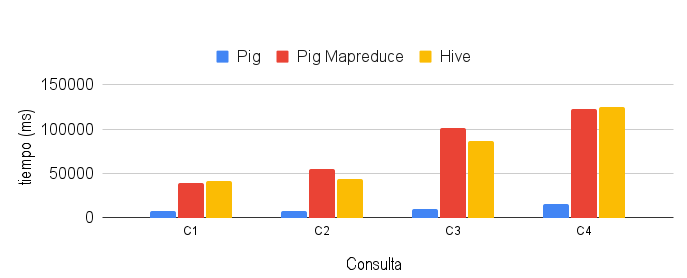
\includegraphics[scale=0.5]{Pig, Pig Mapreduce y Hive (2).png}
	\caption{Gráfico de tiempos de ejecución}
	\label{fig:tiempos}
\end{figure}
\\
En la tabla \ref{tbl:trabajos_mapreduce} se muestra la cantidad de trabajos. En el primer valor los \textit{map} y en el segundo los \textit{reduce}. Se ve que Hive realiza la menor cantidad de tareas para cada consulta, seguido de pig Mapreduce y, finalmente, Pig local es el que más tareas realiza.
\setlength{\tabcolsep}{10pt} % Default value: 6pt
\renewcommand{\arraystretch}{1.5} % Default value: 1
\begin{table}[hp]
	\centering
	\caption{Número de trabajos realizados.\label{tbl:trabajos_mapreduce}}
	\begin{tabular}{llll}
		{Consulta} & Pig local & Pig mapreduce & Hive \\ \hline
		C1                                                      & (3, 1)    & (2, 1)             & (2, 1)    \\
		C2                                                      & (4, 2)    & (3, 2)             & (2, 2)    \\ 
		C3                                & (6, 3)    & (5, 4)             & (4, 3)    \\
		C4                                                      & (8, 4)    & (6, 4)             & (6, 3)       
	\end{tabular}
\end{table}\\
Las respuestas a las consultas son:
\begin{itemize}
	\item \textbf{C3}: Charles Benedict Ainslie y
	Paul Bert Elvstrm. Ambos con cuatro medallas de oro.
	\item \textbf{C4}: Michael Phelps con 28 medallas, 23 de ellas de Oro. Es el mejor por ambos criterios, total de medallas y total de medallas de oro.
\end{itemize}
\section*{Conclusiones}
\addcontentsline{toc}{section}{\protect\numberline{}Conslusiones}
A grandes rasgos, en esta práctica hay dos aspectos importantes a comparar entre Pig y Hive: 
\begin{itemize}
	\item La sintaxis para el desarrollo de consultas o creación de conjuntos de datos.
	\item Eficiencia en el cómputo de las consultas.
\end{itemize}
Respecto a la sintaxis, queda patente que Hive (HQL), por su gran similitud con SQL y legibilidad, es más accesible y cómodo para el público general. Sin embargo, Pig se demuestra más versátil que Hive, y podría integrarse en procesos \textit{batch} para generar nuevos conjuntos de datos desde datos en bruto, al contrario que Hive, que está más orientado a \textit{reporting} y datos ya estructurados. En este aspecto, se concluye que Pig es una herramienta para el entorno técnico mientras que Hive se centra en el entorno funcional de negocio.\\\\
Por otro lado, respecto a la eficiencia de cómputo, el tamaño de los datos no permite llegar a conclusiones claras. Pig local ha sido el más rápido, ya que sobre ficheros de pequeño tamaño, el acceso a disco es mucho más rápido a local que a HDFS. Respecto a Pig mapreduce y Hive, con este experimento no se puede afirmar que uno sea mas eficiente que otro. Sin embargo, no se espera que los tiempos de ejecución aumenten significativamente al variar el tamaño del archivo, algo que en Pig local sí cabe esperar.\\\\
Pese a que se ha realizado en modo \textit{standalone}, no cabe duda que ambas tecnologías constituyen una herramienta muy potente para el tratamiento de datos masivos y, en particular, el punto fuerte es que consiguen dar acceso a un gran público al paradigma mapreduce.
\pagebreak
\section*{\centering{Anexo}}
\addcontentsline{toc}{section}{\protect\numberline{} Anexo}
\begin{figure}[hp!]
	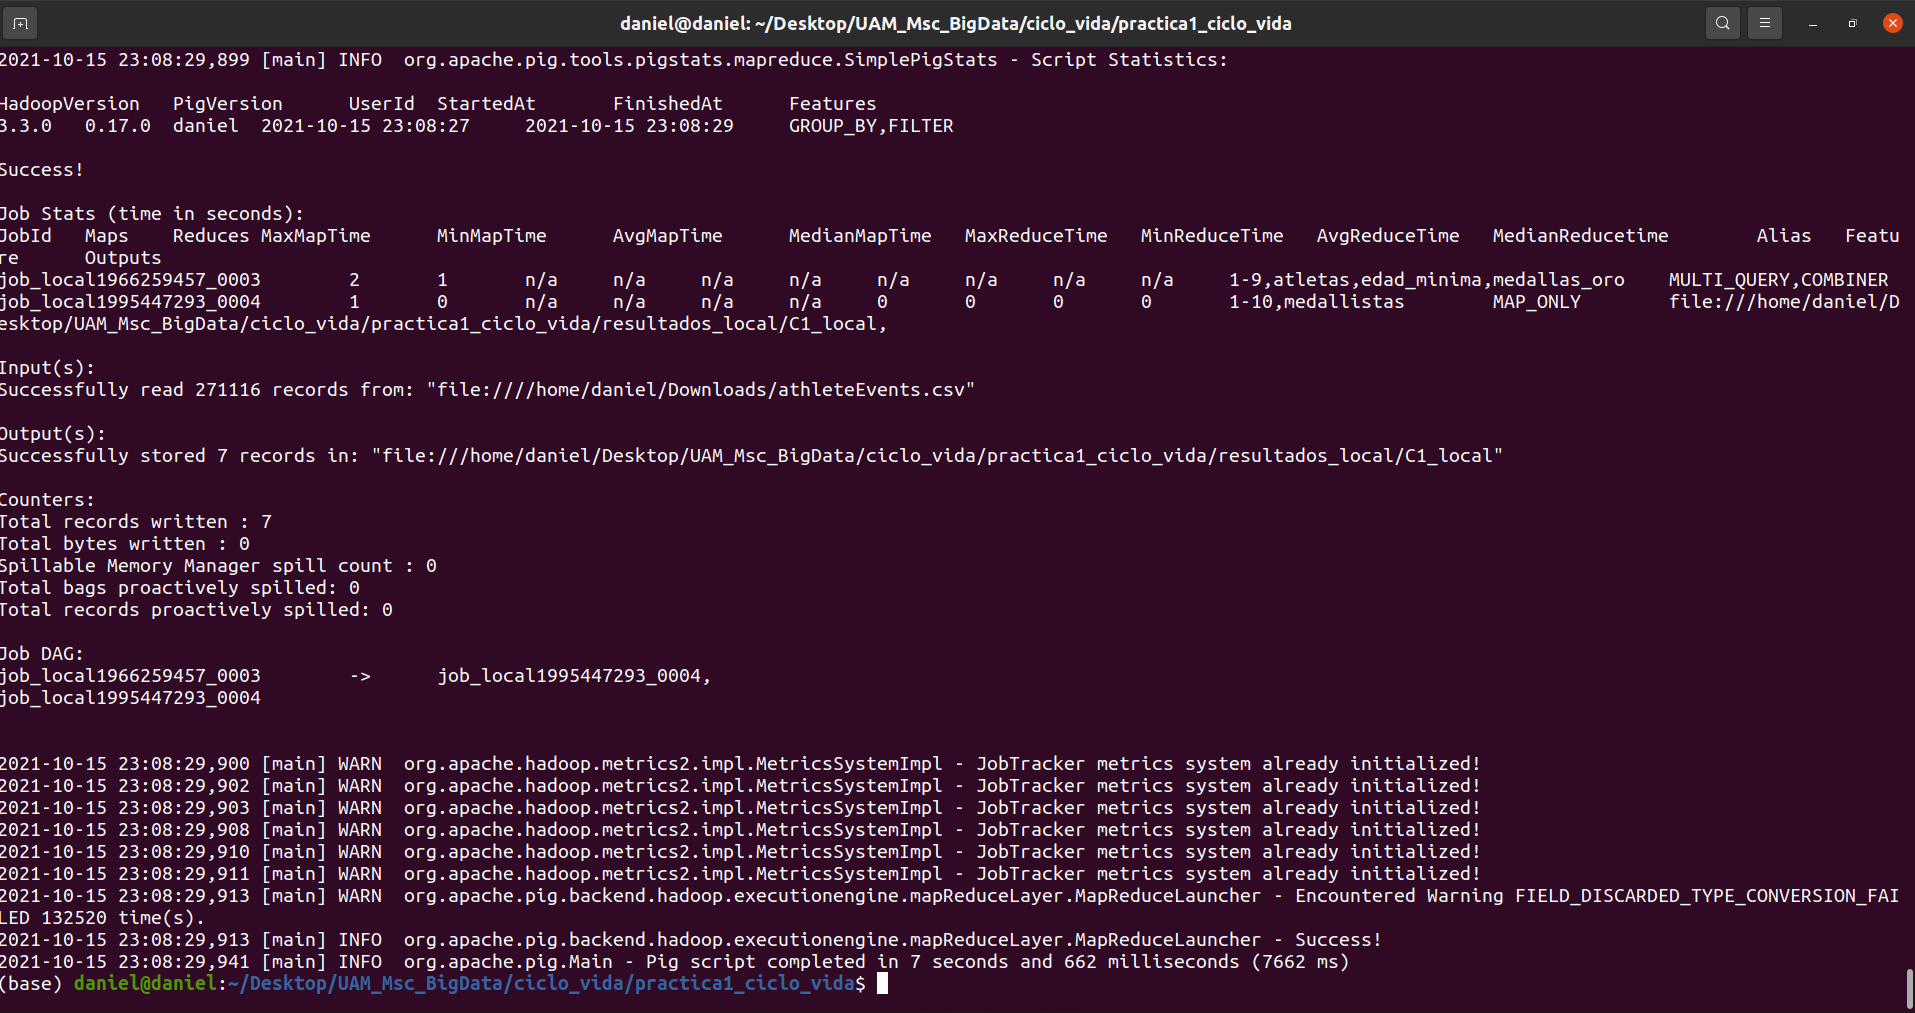
\includegraphics[scale=0.25]{C1_piglocal.png}
	\caption{Salida por consola C1 pig local}
	\label{fig:pig_C1_local}
\end{figure}
\begin{figure}[hp!]
	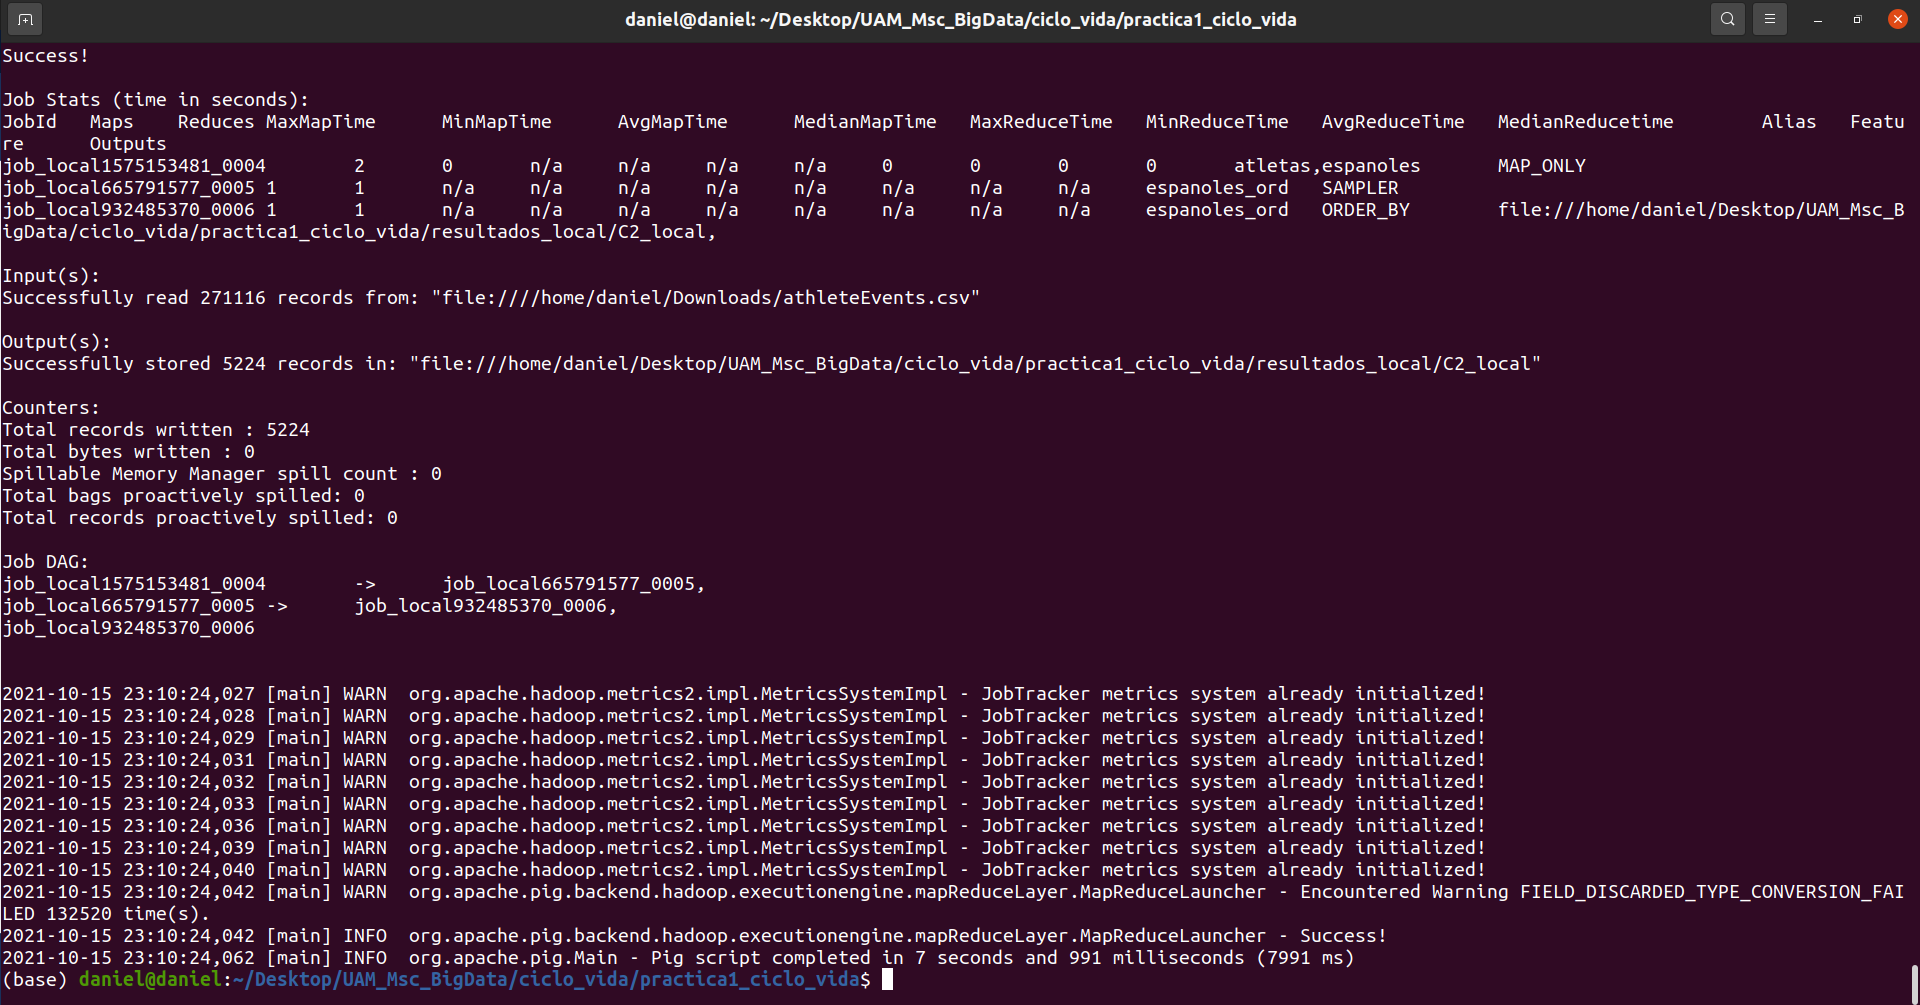
\includegraphics[scale=0.25]{C2_piglocal.png}
	\caption{Salida por consola C2 pig local}
	\label{fig:pig_C2_local}
\end{figure}
\pagebreak
\begin{figure}[hp!]
	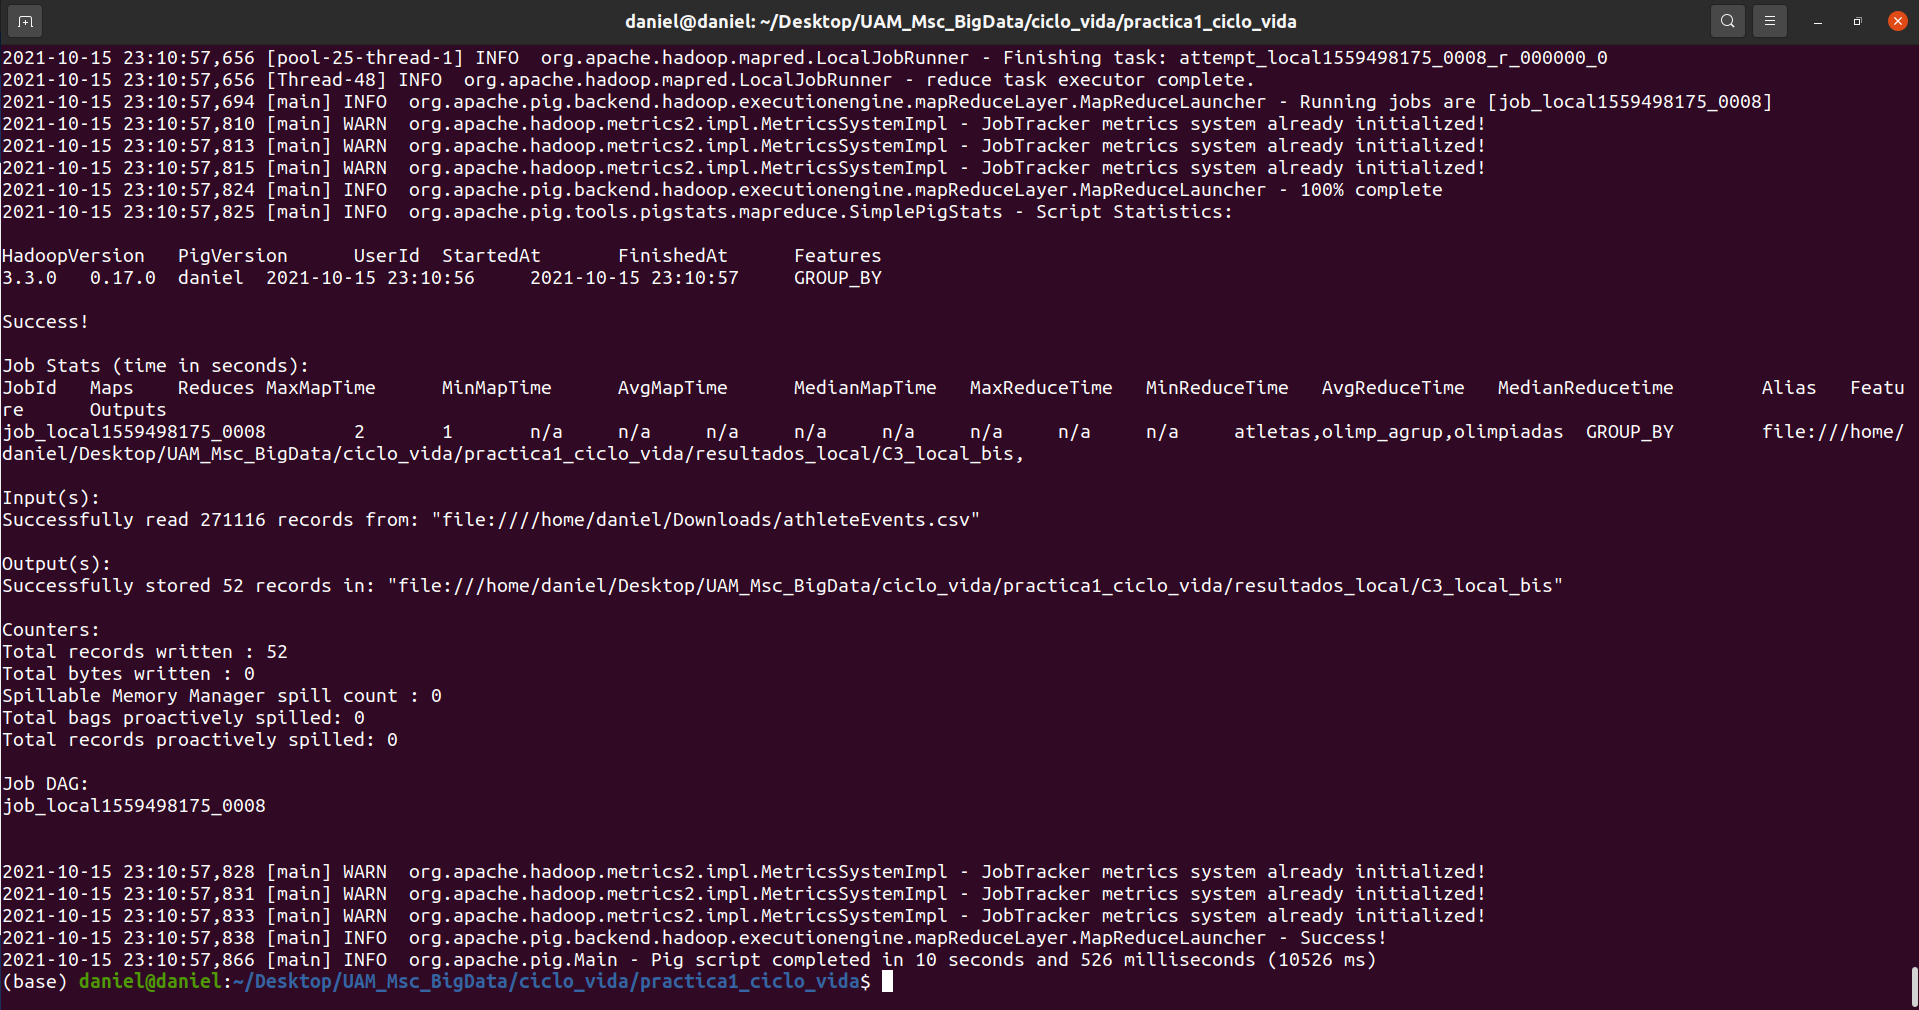
\includegraphics[scale=0.25]{C3_piglocal.png}
	\caption{Salida por consola C3 pig local}
	\label{fig:pig_C3_local}
\end{figure}
\begin{figure}[hp!]
	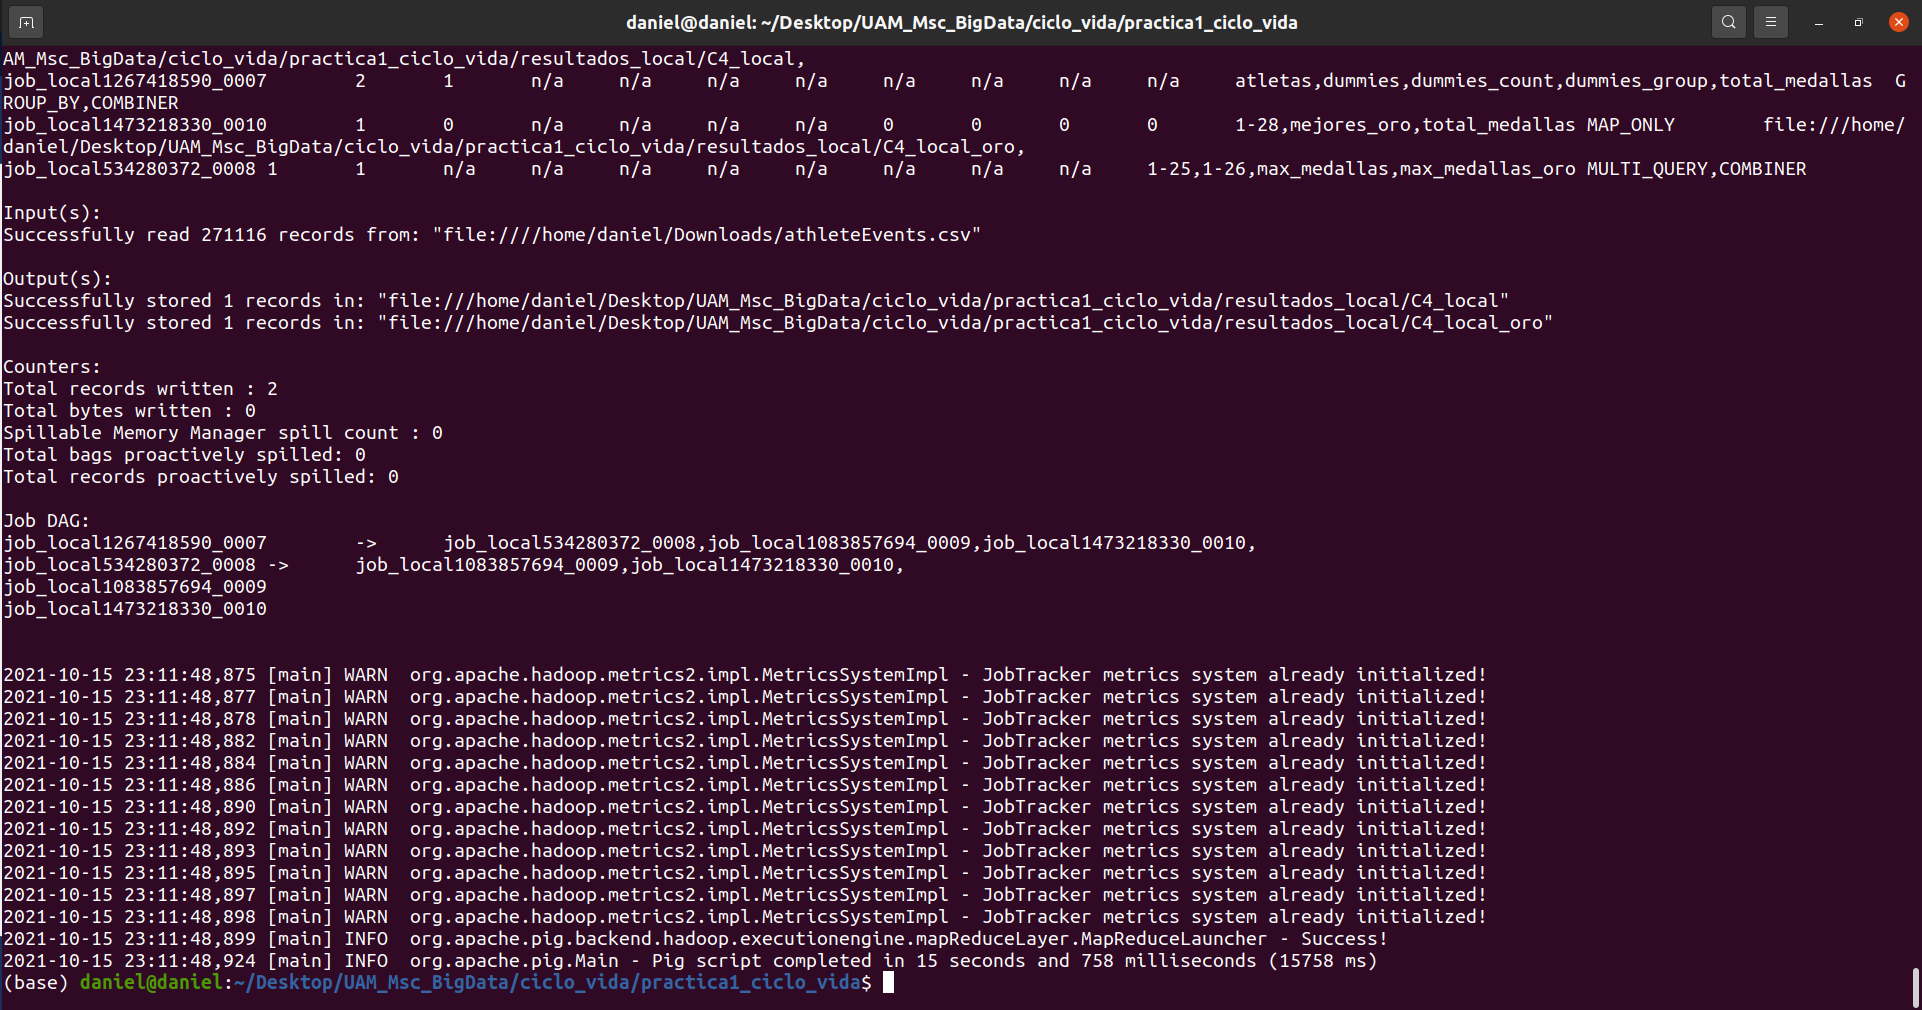
\includegraphics[scale=0.25]{C4_piglocal.png}
	\caption{Salida por consola C4 pig local}
	\label{fig:pig_C4_local}
\end{figure}
\pagebreak
\begin{figure}[hp!]
	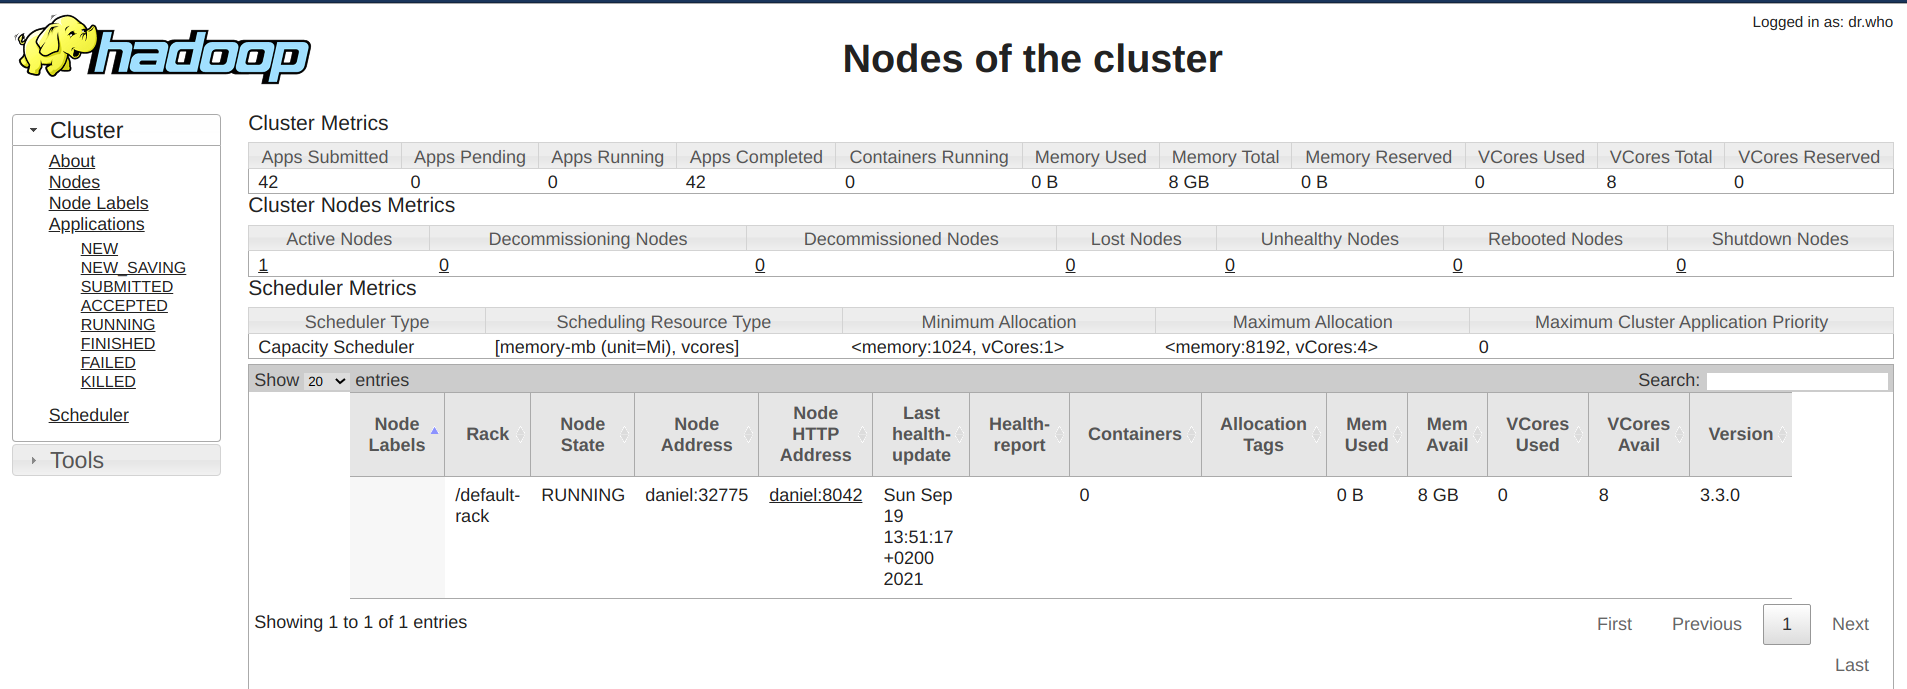
\includegraphics[scale=0.25]{hadoop_cluster.png}
\caption{Resumen del servicio Hadoop funcionando correctamente}
\label{fig:resumen_hadoop}
\end{figure}
\begin{figure}[hp!]
	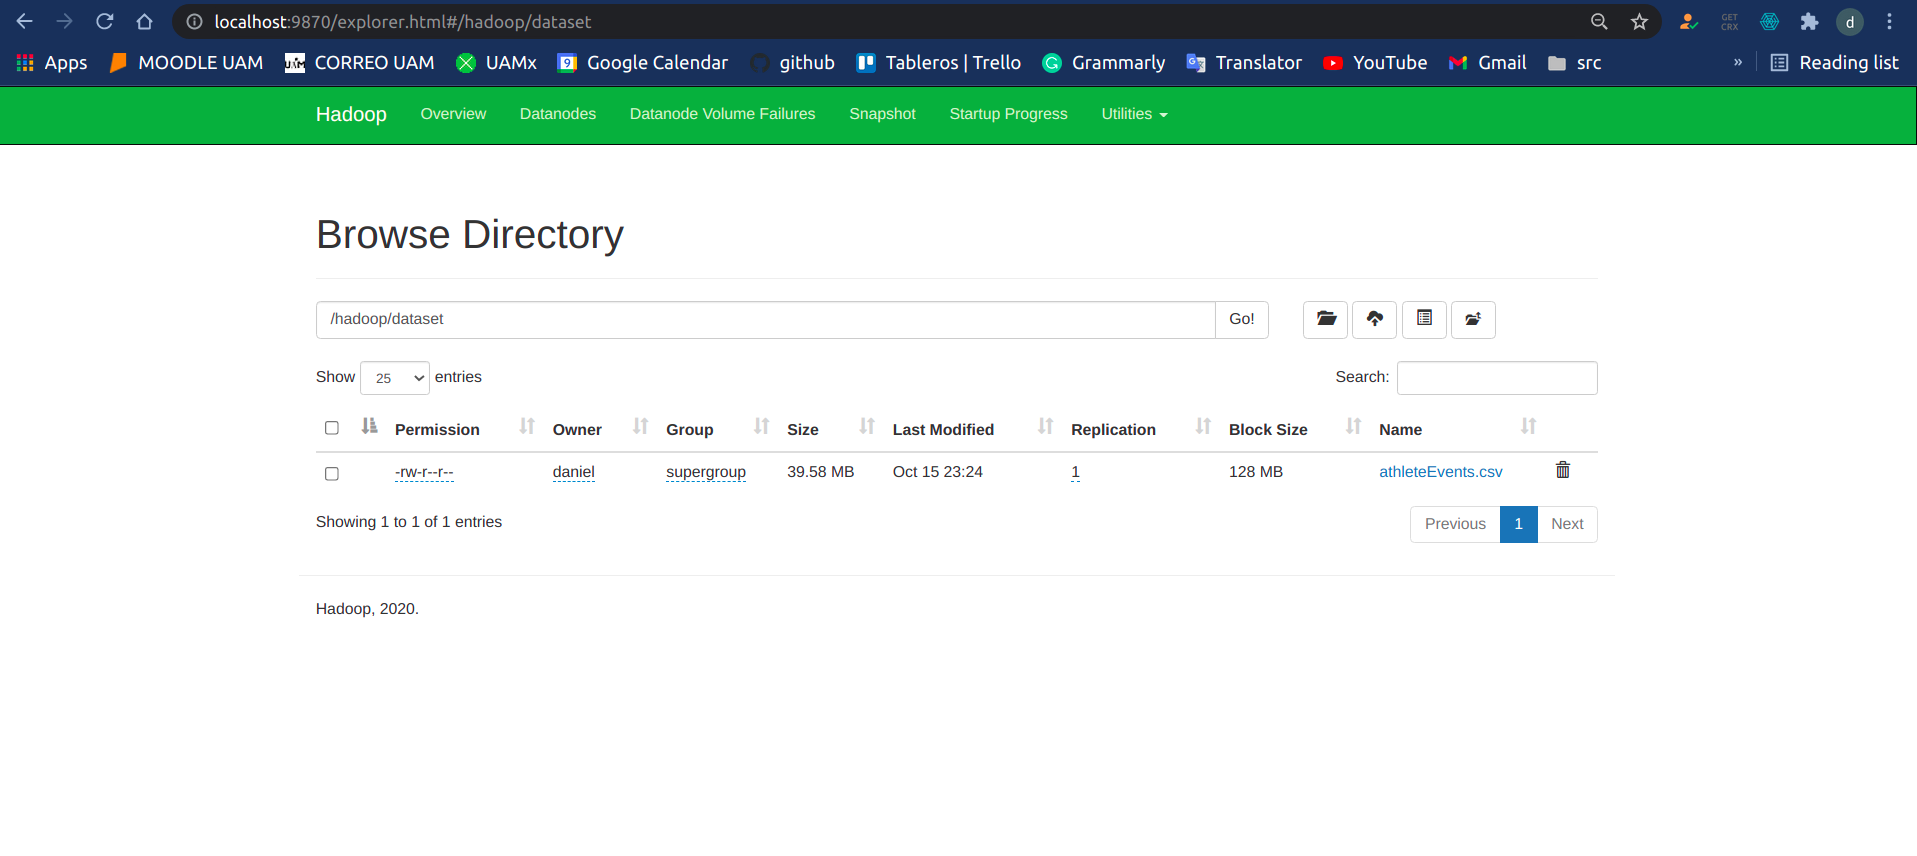
\includegraphics[scale=0.25]{figures/hadoop_dataset.png}
	\caption{ruta a los datos en HDFS}
	\label{fig:datos_HDFS}
\end{figure}
\pagebreak
\begin{figure}[hp!]
	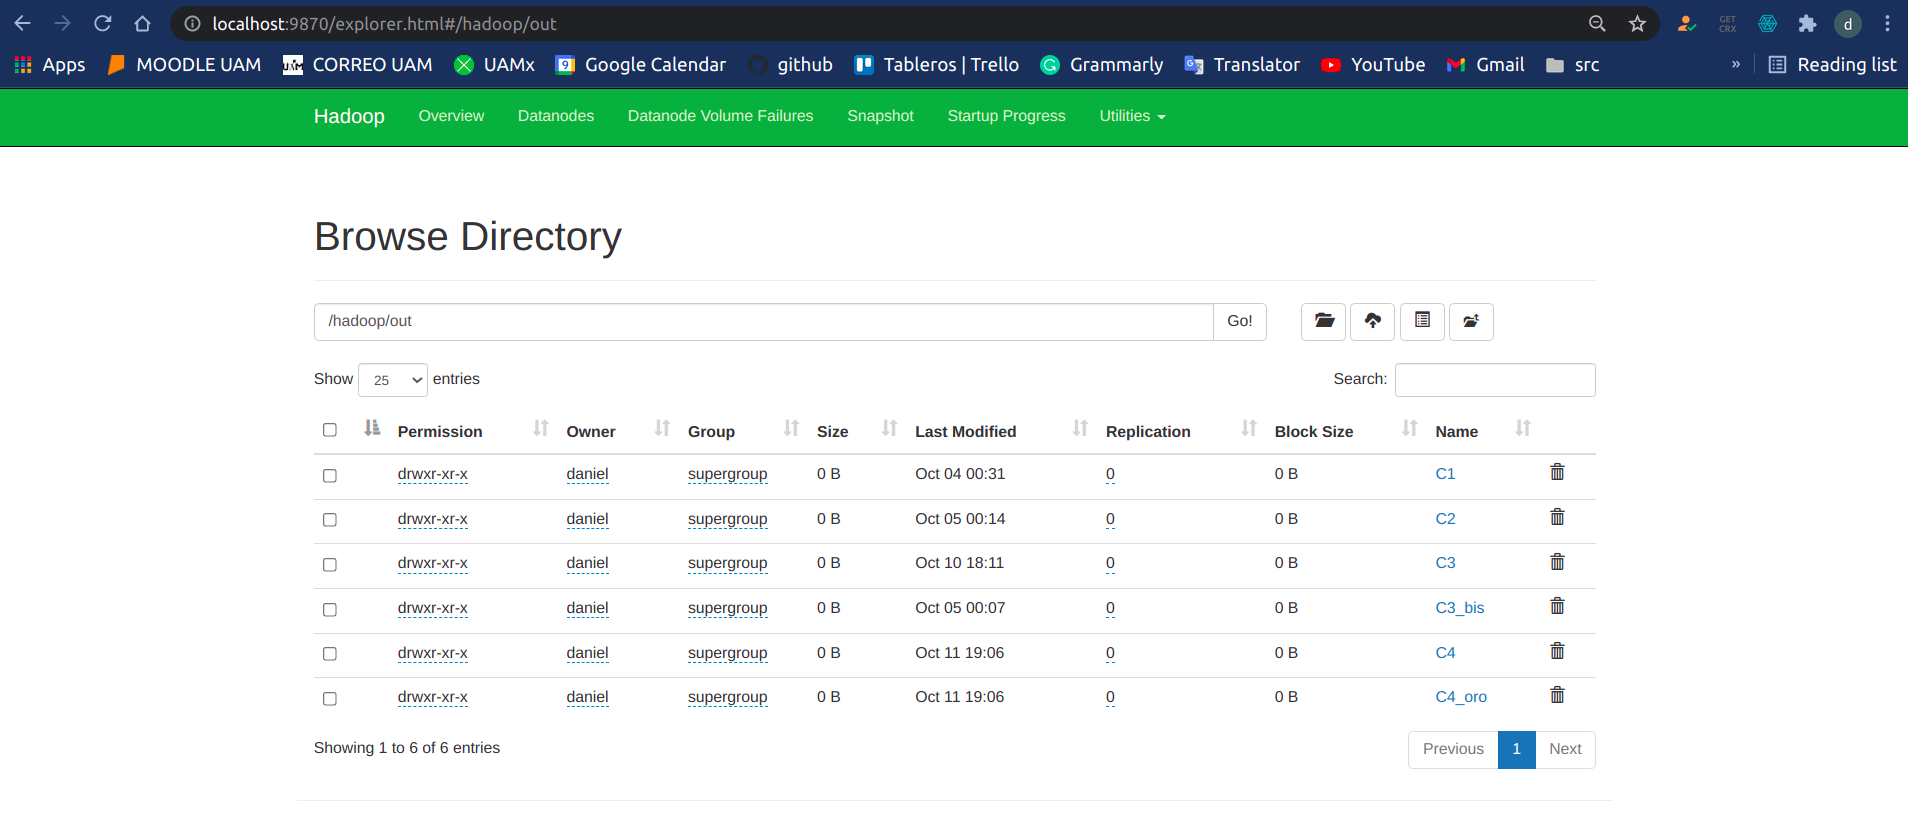
\includegraphics[scale=0.25]{figures/hadoop_out.png}
	\caption{ruta a los resultados de PIG mapreduce en HDFS}
	\label{fig:cruta_out_HDFS}
\end{figure}
\begin{figure}[hp!]
	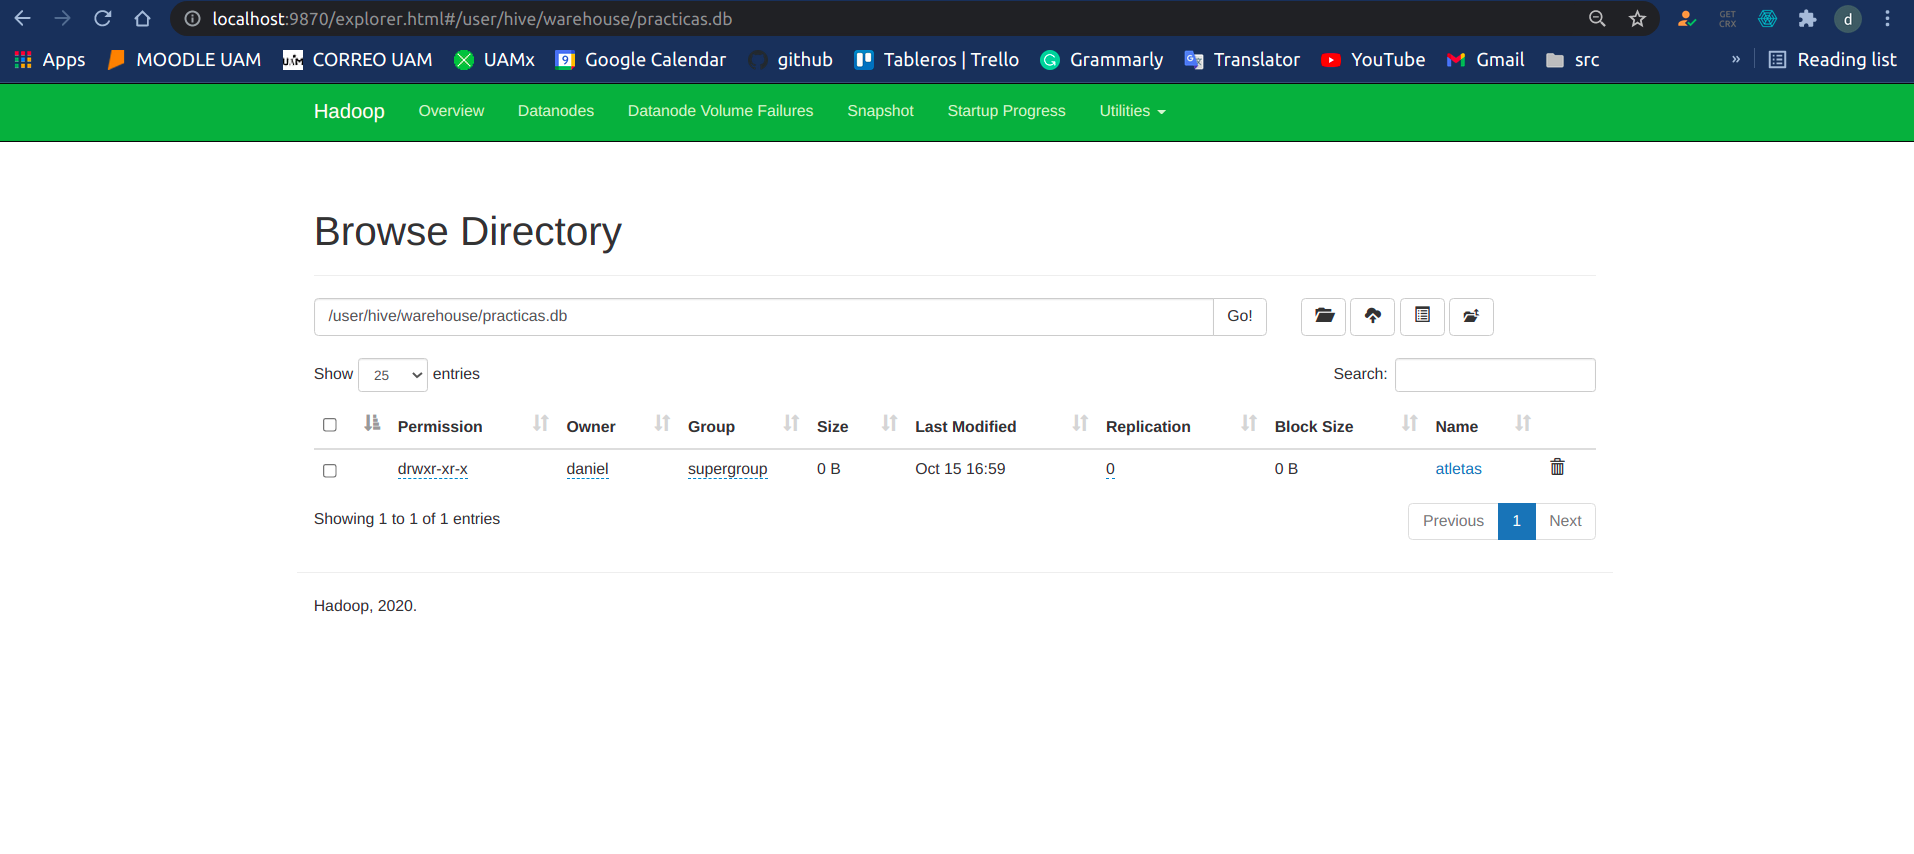
\includegraphics[scale=0.25]{figures/hadoop_practicas.png}
	\caption{Contenido de la base de datos \textit{practicas}}
	\label{fig:practicas}
\end{figure}
\pagebreak
\begin{figure}[hp!]
	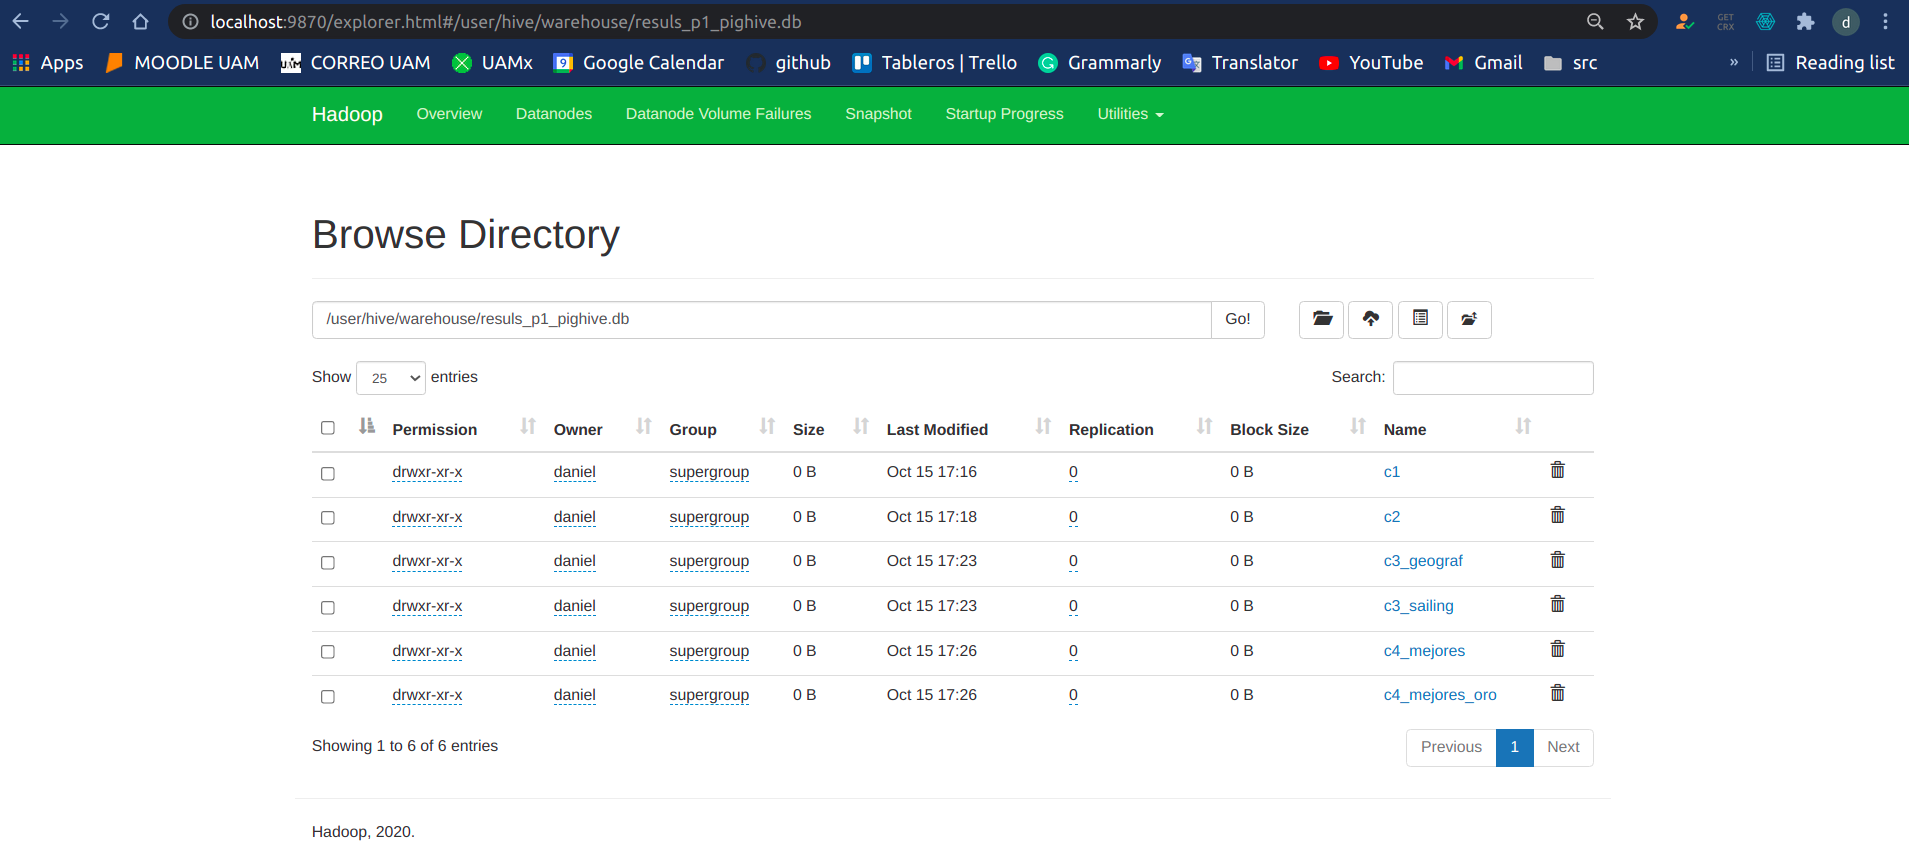
\includegraphics[scale=0.25]{resuls_p1_pighive.png}
	\caption{Contenido de la base de datos \textit{resuls\_p1\_pighive}}
	\label{fig:resuls_hive}
\end{figure}
